\documentclass{article}
\usepackage{graphicx}
\usepackage{hyperref}
\title{BERA-gOHM Thesis and more}
\begin{document}
\maketitle
\section{Introduction}
This article will discuss investment opportunities for Berachain (ticker: \$BERA), an up and coming EVM-compatible L1 built on the Cosmos SDK, and Olympus (tickers: \href{https://dexscreener.com/ethereum/0x893f503fac2ee1e5b78665db23f9c94017aae97d}{\$OHM}, \href{https://dexscreener.com/ethereum/0x08f68110f1e0ca67c80a24b4bd206675610f445d}{\$gOHM}), describing itself as a community-owned, decentralized and censorship-resistant reserve currency.

\

Berachain and Olympus are considered together due to \$gOHM being a possible investment vehicle for the \$BERA token, but also due to the fact that both communities are shown to be tied one to another, more or less.

\

It should also be noted that the Olympus community is currently trying to heavily capitalize on their Berachain investment via intensive social media interaction.

\

We will keep the analysis concise for the sake of brevity.

\newpage
\section{Analysis}

Berachain has last \href{https://cryptonews.com/news/berachain-secures-42-million-series-a-at-42069m-valuation-boosting-defi-focused-layer-1.htm}{been reported} to have a valuation of \$420.69MM.

\begin{figure}[h]
    \centering
    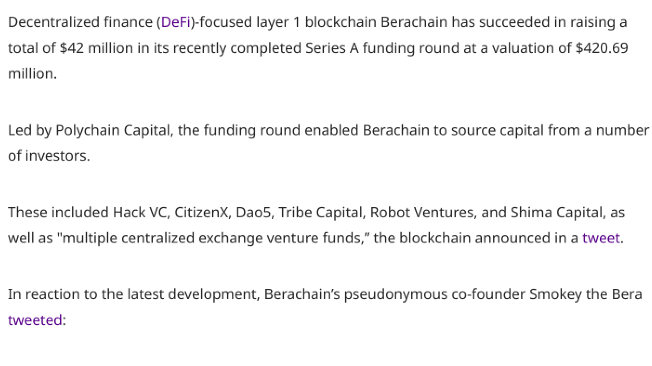
\includegraphics[width=0.9\textwidth]{valuation.png}
    \caption{April 21 2023}
\end{figure}

Olympus has acquired with \href{https://forum.olympusdao.finance/d/1127-oip-87-berachain-investment-strategic-partnership}{OIP-87} 1\% of the total \$BERA supply at a valuation of \$50MM.

\begin{figure}[h]
    \centering
    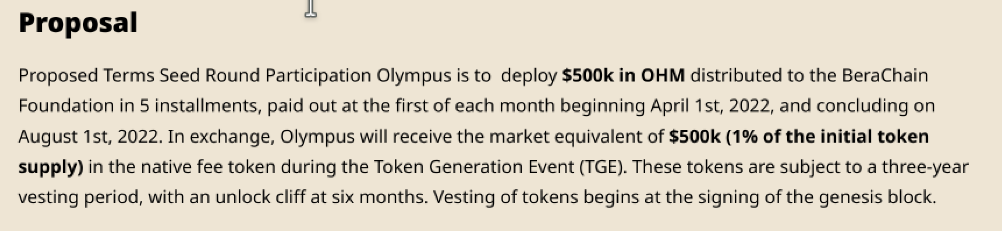
\includegraphics[width=1\textwidth]{bera.png}
    \caption{The passed OIP-87 investment}
\end{figure}


Olympus \$BERA is subject to a 3 year vesting period with a 6 month cliff according to the \href{https://x.com/zeetientien/status/1704845265956438046?s=20}{following Tweet made by an Olympus community member.}

\newpage

\begin{figure}[h]
    \centering
    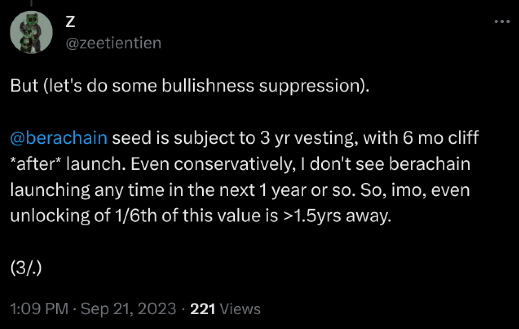
\includegraphics[width=0.75\textwidth]{vesting.png}
    \caption{Olympus \$BERA is subject to a vesting period}
\end{figure}

Olympus is also in the process of modifying Cooler Loan\footnotemark[1] and RBS\footnotemark[2] parameters with \href{https://forum.olympusdao.finance/d/4048-oip-149-backing-ratification-for-cooler-loans-and-rbs}{OIP-149.}

\begin{figure}[h]
    \centering
    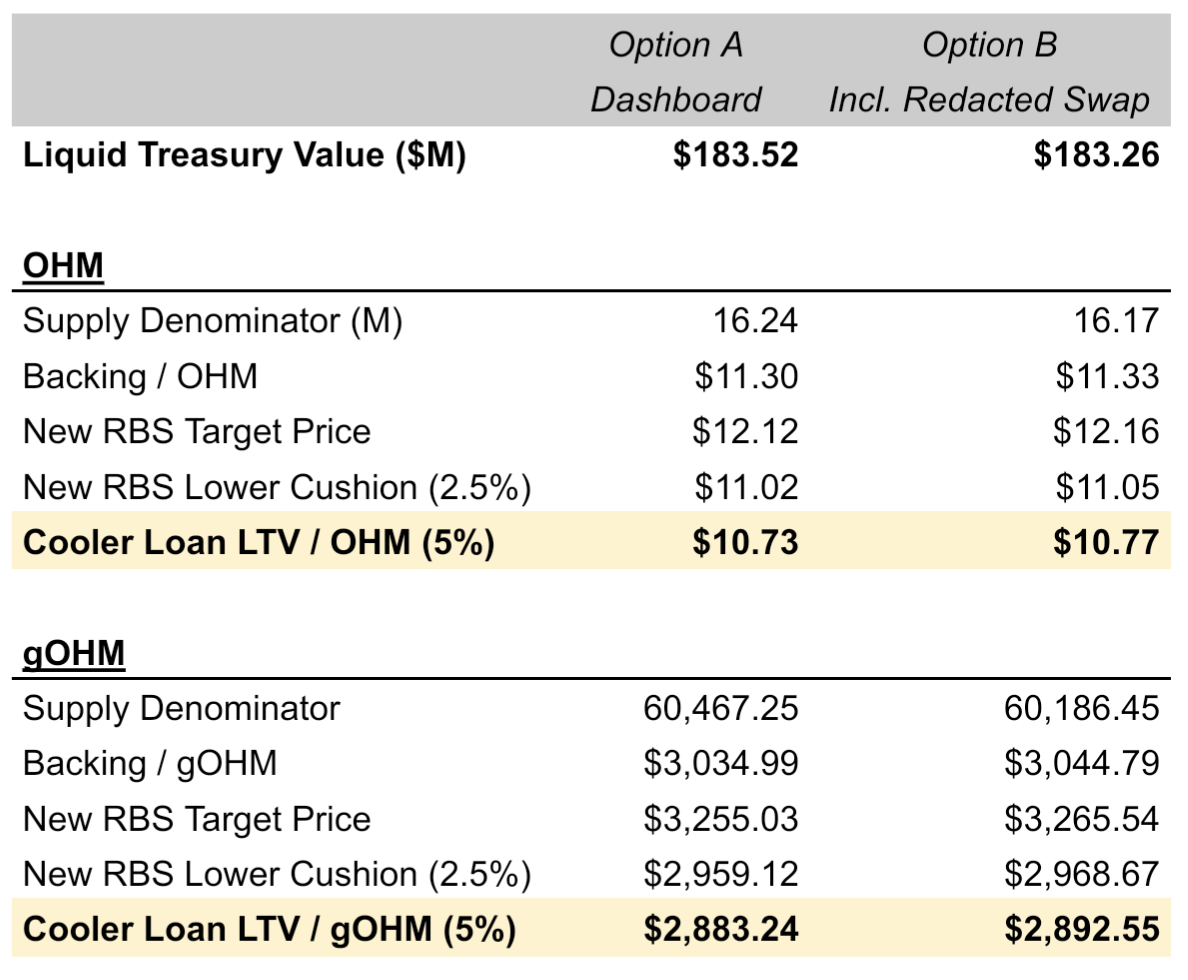
\includegraphics[width=0.65\textwidth]{zpost1.png}
    \caption{OIP-149 proposed parameters}
\end{figure}

\

All of the former implies that assuming the lower bounds of Cooler Loans and RBS hold, there is a way to calculate the maximum risk free leveraged dollar investment amount based on the Berachain valuation.

\footnotetext[1]{"Cooler Loans" are fixed-term (4 months), fixed-rate (0.5\%), fixed-price DAI for gOHM loans. }

\newpage

\footnotetext[2]{Or "Range Bound Stability", an algorithmic market making system which maintains the price of OHM within a certain range by utilizing Olympus treasury assets. Read: at the lower bound of some price interval, which we will later call $p_l$, RBS buys back \$OHM tokens, meaning that these tokens are at a discount if $p_{OHM} < p_l$ }

Let us denote with $I_0$ the dollar valuation of our \$gOHM investment before leverage, $I_n$ the value of our total \$gOHM collateral after $n$ rounds of leverage, $m_v$ the \$BERA valuation multiplier, meaning the multiplier of the current \$BERA valuation based on an initial \$50MM valuation, and lastly $m_s$, our share of the total valuation, this is based on the market cap ($m_s = I_n / MC$).

\

Since Cooler Loans are 95\% LTV, and since we are borrowing at a fixed price, we can borrow only less than 95\% LTV. But also,  this means, the price itself regulates the LTV when it is above the boundary prices mentioned above. Let us denote the current market price with $p_m$ and the lower Cooler Loan OR RBS price with $p_l$. Let us also denote some lower dollar amount bound $B$ below which we will not leverage further. Then our leveraged position will satisfy:

\begin{equation}
    LTV = 0.95 * (p_l / p_m)
\end{equation}

After $n$ rounds of leveraging, there should be only $B$ funds left which may be reused for further collateral.

\begin{equation}
    I_0 * LTV^n = B
\end{equation}

(3), (4) are transformations:

\begin{equation}
    LTV = \sqrt[n]{B/I_0}
\end{equation}

\begin{equation}
    \log_{B/I_0}(LTV) = 1 / n
\end{equation}

We receive our number of leveraging rounds:

\begin{equation}
    n = \frac{1}{\log_{B/I_0}(LTV)}
\end{equation}

For computing:

\begin{equation}
    n = \lfloor\frac{ln(B/I_0)}{ln(LTV)}\rfloor
\end{equation}

The following is a mathematical identity:

\begin{equation}
    I_n = I_0 * \frac{LTV^{n+1} - 1}{LTV - 1}
\end{equation}

\newpage

We should satisfy:

\begin{equation}
    I_n * (1 - p_l / p_m) < m_v * m_s * \$50MM
\end{equation}

(9), (10), transformations:

\begin{equation}
    I_n  < \frac{m_v * m_s * \$50MM}{1 - p_l / p_m}
\end{equation}

\begin{equation}
    I_0 * \frac{LTV^{n+1} - 1}{LTV - 1}  < \frac{m_v * m_s * \$50MM}{1 - p_l / p_m}
\end{equation}

Finally:

\begin{equation}
    I_0 <  \frac{m_v * m_s * \$50MM * (LTV - 1)}{(1 - p_l / p_m)*(LTV^{n+1} - 1)}
\end{equation}

\

Find the largest $I_0$ for which above holds ($n$, $m_v$, $m_s$ also have to be varied).

\

\section{Example}

\

Let us assume a max valuation of \$500MM, in other words $m_v = 10.$ Currently, $MC = \$200MM$. Let us assume a lower bound as stated in Figure 4, we will assume RBS lower cushion from Option A, so $p_l = \$2,959.12$. Price as of the time of writing $p_m = \$3,094.79$. Ratio: $p_l / p_m \approx 0.956162$. Thus, $LTV = 0.908354$.

\

$I_0 = \$100,000$, $B = \$1000$. Thus, $n = 47$. This leads to $I_{47} = \$1,080,336$. A million borrowed! $m_s \approx 0.005402$.

\

Is the condition fulfilled (posting only results)? Yes!

\

\begin{equation}
\$100,000 < \$570,315
\end{equation}

\

Anything below $m_v = 1.7534$ is not enough though.


\end{document}

